\section{Hadronic Results}
\begin{frame}{Hadronic Results - Unpolarized vs. Polarized}
\begin{center}
unpolarized $\sim$ MSTW2008 $\leftrightarrow$ polarized $\sim$ DSSV2014\quad\,\,\,\\
\quad\quad\quad\iRef{Martin,Stirling,Thorne,Watt} $\leftrightarrow$ \iRef{de Florian,Sassot,Stratmann,Vogelsang}
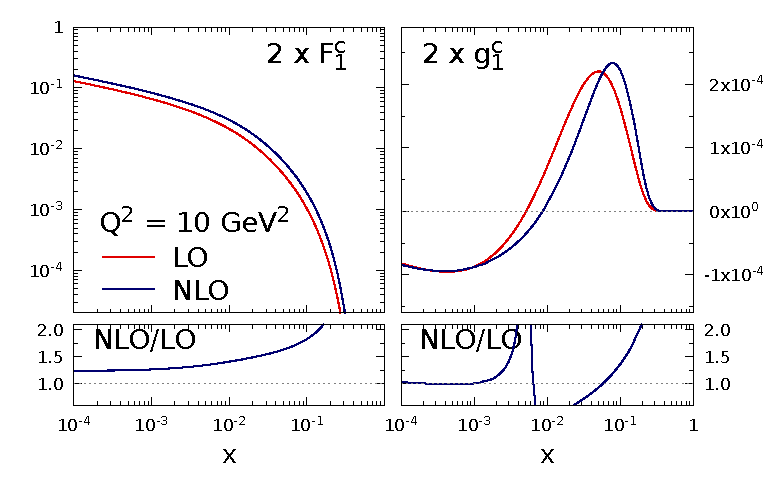
\includegraphics[width=.8\textwidth]{img/F1g1}
\end{center}
\end{frame}

\begin{frame}{Hadronic Results - PDF Uncertainties DSSV (I)}
\newcolumntype{w}{>{\centering\arraybackslash} m{.60\linewidth} }
\newcolumntype{n}{>{\centering\arraybackslash} m{.39\linewidth} }
\begin{tabular}{wn}
\begin{center}
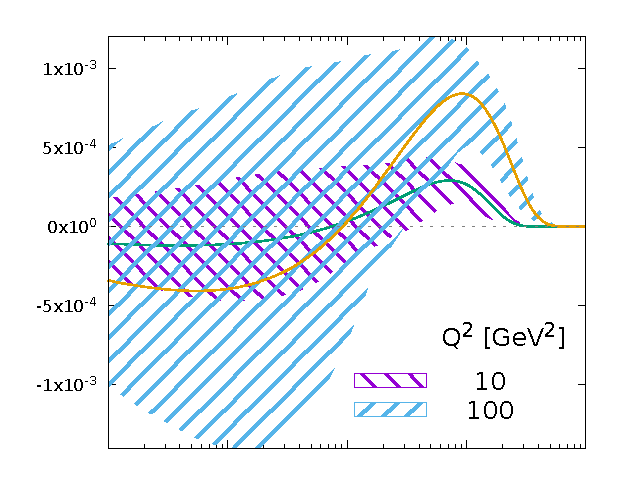
\includegraphics[width=.65\textwidth]{img/g1NLO-pdf}
\end{center} & 
\begin{itemize}
\item quark error band is small
\item sign unconstrained
\item gluon dominates (?)
\item default gluon is small
\end{itemize}
\end{tabular}
\end{frame}

\begin{frame}{Hadronic Results - PDF Uncertainties DSSV (II)}
\newcolumntype{w}{>{\centering\arraybackslash} m{.5\linewidth} }
\newcolumntype{n}{>{\centering\arraybackslash} m{.5\linewidth} }
\begin{tabular}{wn}
\begin{center}
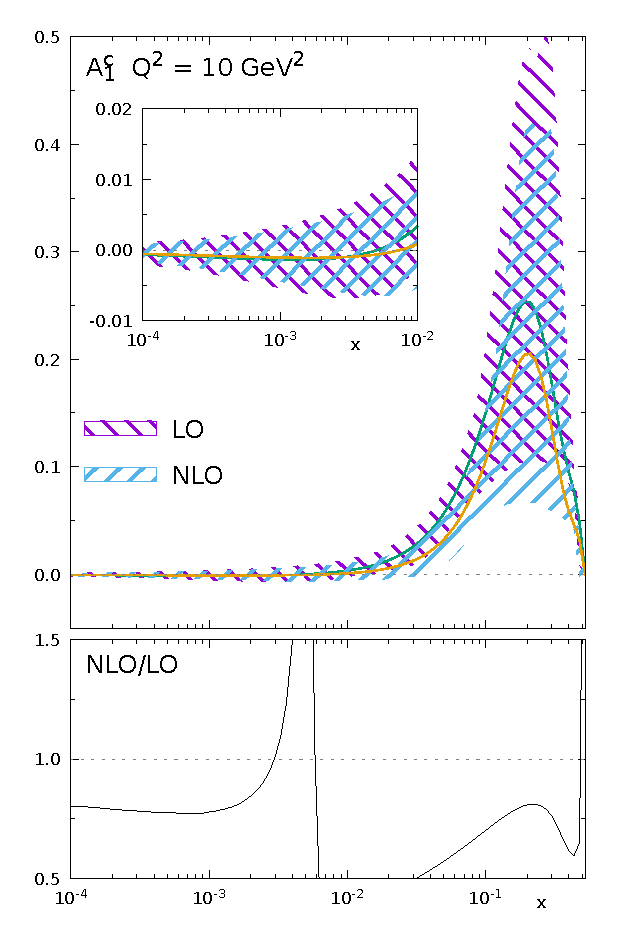
\includegraphics[height=.97\textheight]{img/A1-pdf}
\end{center} & 
\begin{itemize}
\item $A_1^c(x,Q^2) = \frac{g_1^c(x,Q^2)}{F_1^c(x,Q^2)}$
\item error band are only due to DSSV uncertainties (no correlations!)
\invisible{
\item sign unconstrained
\item need measurement of $\mathcal O(10^{-3})$
\item NLO $\lessapprox$ LO}
\end{itemize}
\end{tabular}
\end{frame}
\begin{frame}{Hadronic Results - PDF Uncertainties DSSV (II)}
\newcolumntype{w}{>{\centering\arraybackslash} m{.5\linewidth} }
\newcolumntype{n}{>{\centering\arraybackslash} m{.5\linewidth} }
\begin{tabular}{wn}
\begin{center}
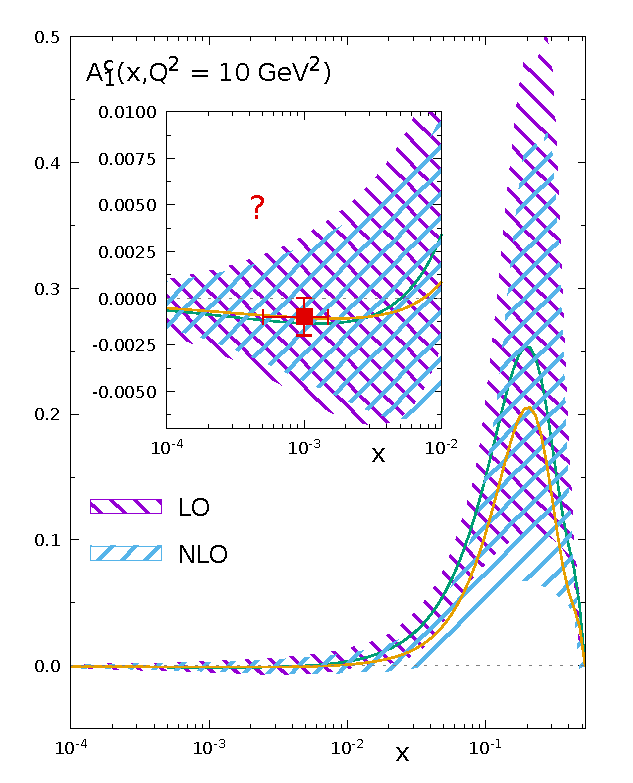
\includegraphics[height=.97\textheight]{img/A1-pdf-data}
\end{center} & 
\begin{itemize}
\item $A_1^c(x,Q^2) = \frac{g_1^c(x,Q^2)}{F_1^c(x,Q^2)}$
\item error band are only due to DSSV uncertainties (no correlations!)
\item sign unconstrained
\item need measurement of $\mathcal O(10^{-3})$
\item NLO $\lessapprox$ LO
\end{itemize}
\end{tabular}
\end{frame}

\begin{frame}{Hadronic Results - Scale Uncertainties (I)}
\begin{center}
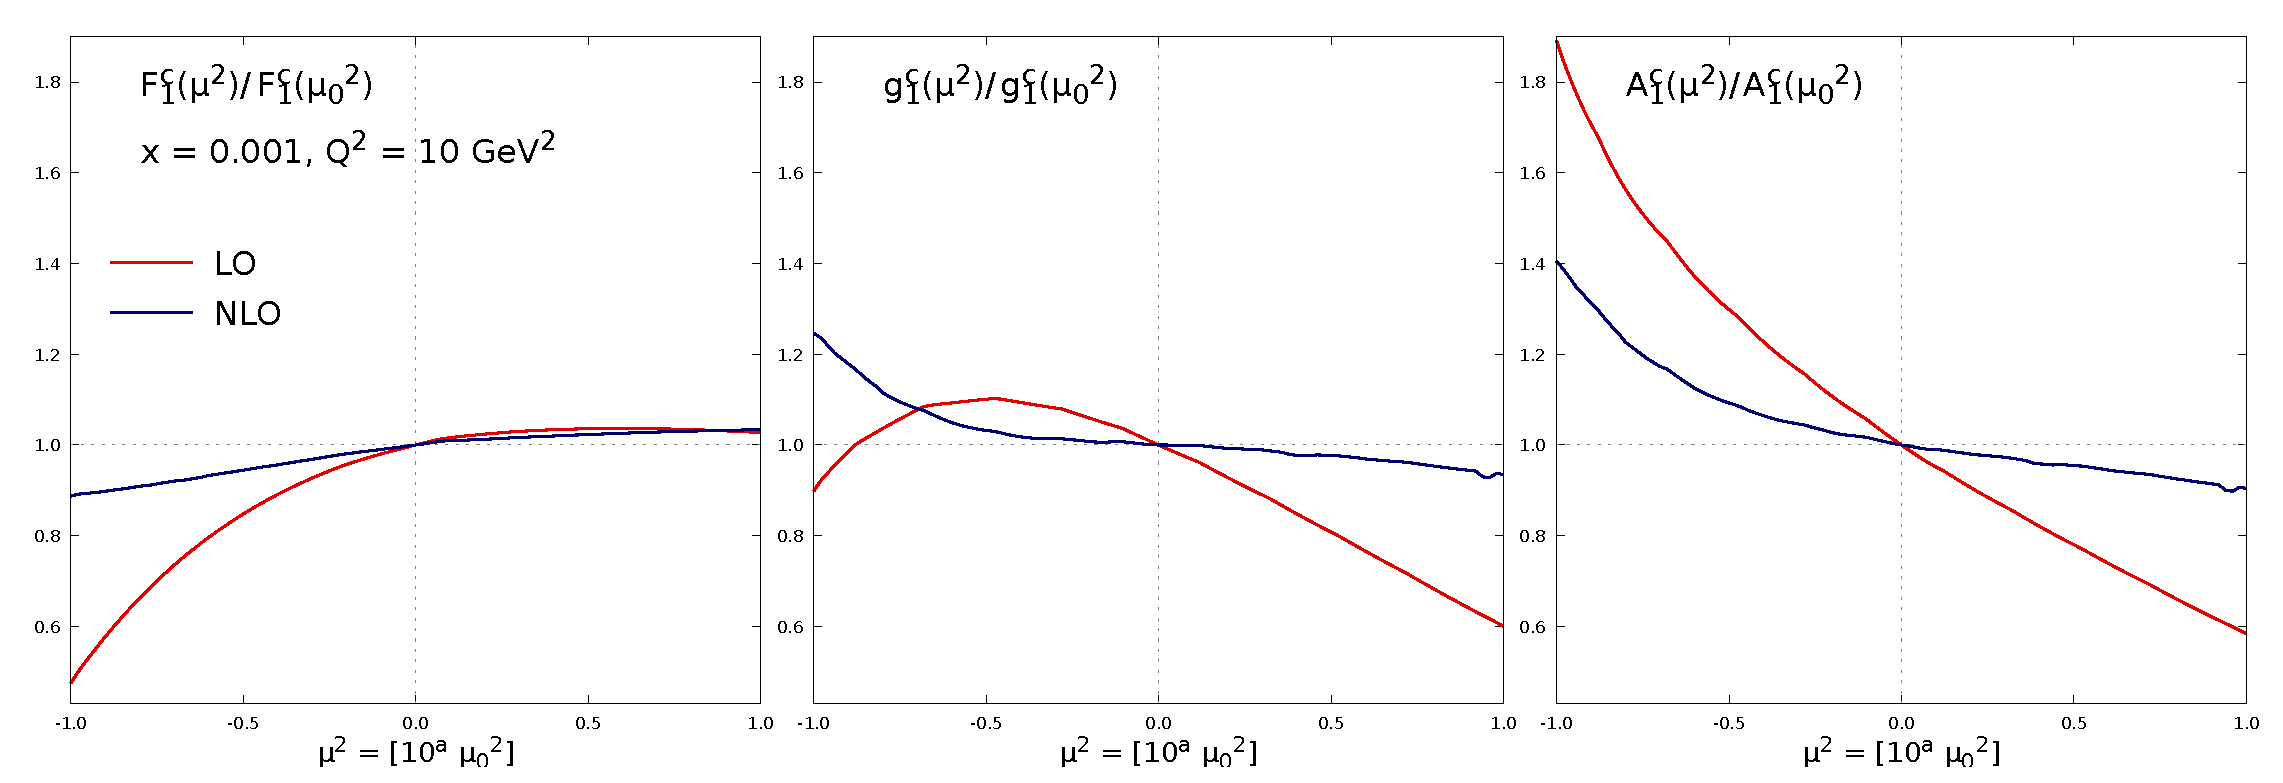
\includegraphics[width=\textwidth]{img/F1g1A1-mu2}
\end{center}
\[\mu_F^2 = \mu_R^2 = 10^a\mu_0^2\,\text{with}\,\mu_0^2=4m^2+Q^2\]
\end{frame}

\begin{frame}{Hadronic Results - Scale Uncertainties (II)}
\begin{center}
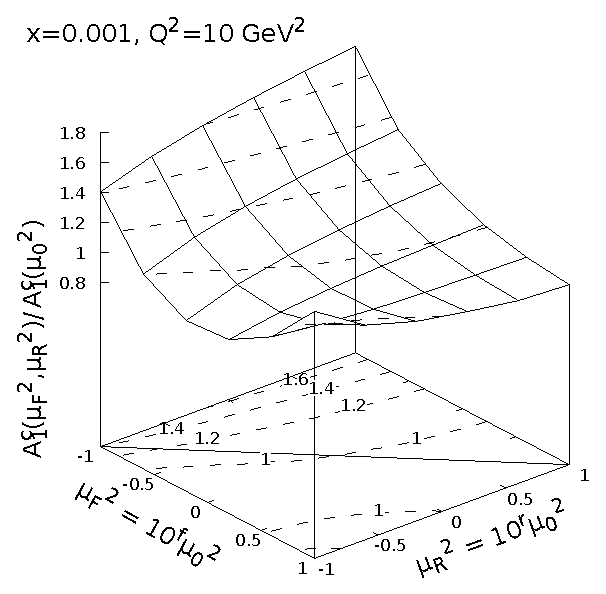
\includegraphics[width=.48\textwidth]{img/A1-muF2-muR2-x_3-q2_1}
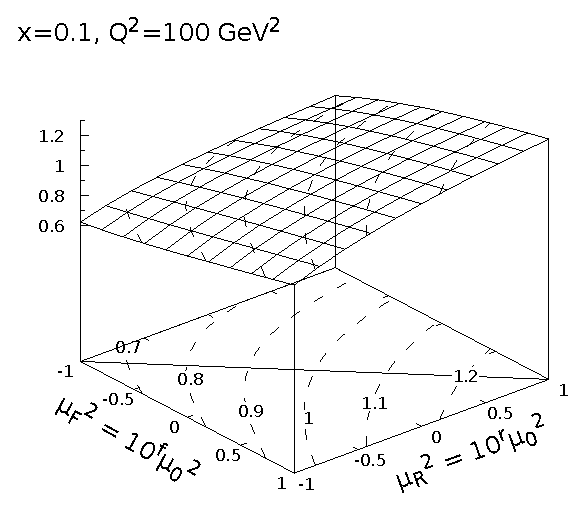
\includegraphics[width=.48\textwidth]{img/A1-muF2-muR2-x_1-q2_2}
\end{center}
\[\mu_0^2=4m^2+Q^2\]
\end{frame}
